\documentclass{beamer}
\special{landscape}

\usetheme{Warsaw}

%\usecolortheme{seahorse}
%\usefonttheme[onlysmall]{structurebold}

\setbeamertemplate{headline}[split]
\setbeamertemplate{footline}[default]
\setbeamertemplate{footline}[miniframes theme]
%\logo{\includegraphics[scale=0.25]{lifia_logo.png}}

\mode<presentation>
\usepackage[spanish]{babel}
\usepackage{beamerthemesplit}
\usepackage{color}      % use if color is used in text

\usepackage[utf8]{inputenc}

% Comandos en modo Verbatim
%\usepackage{fancyvrb}

\usepackage{listings}


%%
%% WinMIPS64 definition (c) 2020
\lstdefinelanguage{WinMIPS64}
 {morekeywords={%
cvt.l.d,cvt.d.l,mfc1,mtc1,DADD,DADDI,ANDI,XORI,HALT,BEQ,BNEQ,LD,NOP,DMUL,DSUB,AND,DDIV,%
	JAL,J,DSLL,BNEZ,SD, JR, BEQZ, cvt.d.l, cvt.l.d, lwu},%
 otherkeywords={.word,.code,.data,.text, .asciiz, .ascii, .word32 },%
   sensitive=false,%
   morecomment=[l]{;},%
   morestring=[b]",%
 }

\lstset{emph={%  
    F0,F1,F2,F3,F4,F5,F6,F7,F8,F9,F10,F11,F12,F13,F14,F15,F16,F17,F18,F19%
    F20,F21,F22,F23,F24,F25,F26,F27,F28,F29,F30,F31%
    f0,f1,f2,f3,f4,f5,f6,f7,f8,f9,f10,f11,f12,f13,f14,f15,f16,f17,f18,f19%
    f20,f21,f22,f23,f24,f25,f26,f27,f28,f29,f30,f31%
    R0,R1,R2,R3,R4,R5,R6,R7,R8,R9,R10,R11,R12,R13,R14,R15,R16,R17,R18,R19%
    R20,R21,R22,R23,R24,R25,R26,R27,R28,R29,R30,R31%
    r0,r1,r2,r3,r4,r5,r6,r7,r8,r9,r10,r11,r12,r13,r14,r15,r16,r17,r18,r19%
    r20,r21,r22,r23,r24,r25,r26,r27,r28,r29,r30,r31%
	$0,$zero,$s0,$s1,$s2,$s3,$s4,$s5,$s6,$s7,$sp,$ra,$t1%
    },emphstyle={\color{red}\bfseries}%
}%

%\lstset{emph={%  
%    .code,.data,.word
%    },emphstyle={\color{green}\bfseries}%
%}%
\title{Practica 5 - WinMIPS64 - Pila}

\title{Practica 4 - WinMIPS64}
%\author{Juan Antonio Zubimendi\\azubimendi@lifia.info.unlp.edu.ar}

\AtBeginSection[]

\begin{document}

\section{Atascos}

\subsection{Introducción}
\begin{frame}
\frametitle{Introducción}
Suposiciones:
\begin{itemize}
\item Todas las tareas duran el mismo tiempo.
\item Las instrucciones siempre pasan por todas las etapas.
\item Todos las etapas pueden ser manejadas en paralelo.
\end{itemize}
\end{frame}

\begin{frame}
\frametitle{Algunos Problemas}
Problemas:
\begin{itemize}
\item  No todas las instrucciones necesitan todas las etapas
\begin{itemize}
\item \emph{SW RT, inmed(RS)} -  no utiliza W
\item En MSX88 \emph{MOV AX, mem} no requiere EX
\end{itemize}
 \item No todas las etapas pueden ser manejadas en paralelo.
\begin{itemize}
\item F y M acceden a memoria
\end{itemize}
\item No se tienen en cuenta los saltos de control.
\end{itemize}
\end{frame}


\begin{frame}
\frametitle{Atascos}
Llamamos \emph{atasco} a la situación que impide a una o mas instrucciones seguir su camino en el cauce.

\begin{itemize}
\item Estructural
\begin{itemize}
\item Provocados por conflictos con los recursos.
\end{itemize}


\item Dependencia de Datos
\begin{itemize}
\item Dos instrucciones se comunican por medio de un dato
\end{itemize}

\item Dependencia de Control
\begin{itemize}
\item La ejecución de una instrucción depende de cómo se ejecute otra
\end{itemize}

\end{itemize}
Si resolvemos con paradas del cauce, disminuye el rendimiento teórico
\end{frame}


\section{Atascos Estructurales}

\begin{frame}[fragile]
\frametitle{Atascos Estructurales}
Dos o mas instrucciones necesitan utilizar el mismo recurso hardware en el mismo ciclo.

\begin{block}{}
\begin{lstlisting}[language=WinMIPS64,basicstyle=\ttfamily,keywordstyle=\color{blue}]
.text
dmul r7,r7,r3
nop 
nop 
nop 
nop 
nop 
halt
\end{lstlisting}
\end{block}
\end{frame}

\begin{frame}[fragile]
\frametitle{Atasco Estructural}
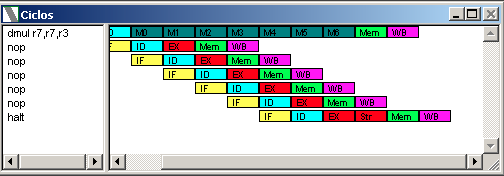
\includegraphics[scale=0.45]{atasco-estructural.png}
\end{frame}


\section{Atascos por dependencia de Datos}
\subsection{General}

\begin{frame}
\frametitle{Atasco por Dependencia de Datos}

Condición en la que los operandos fuente o destino de una instrucción no están disponibles en el momento en que se necesitan en una etapa determinada del cauce.
\begin{itemize}

\item Lectura después de Escritura (RAW, dependencia verdadera)
\begin{itemize}
\item  una instrucción genera un dato que lee otra posterior
\end{itemize}

\item Escritura después de Escritura (WAW, dependencia en salida)
\begin{itemize}
\item una instrucción escribe un dato después que otra posterior
\item sólo se da si se deja que las instrucciones se adelanten unas a otras
\end{itemize}

\item Escritura después de Lectura (WAR, antidependencia)
\begin{itemize}
\item una instrucción modifica un valor antes de que otra anterior que lo tiene que leer lo lea
\item Es el que menos suele darse
\end{itemize}
\end{itemize}
\end{frame}

\subsection{RAW - Lectura luego de una Lectura}
\begin{frame}[fragile]
\frametitle{RAW}
Una instrucción depende del resultado de otra instrucción que todavía no ha finalizado y debe esperar a que el resultado este disponible.
\begin{block}{}
\begin{lstlisting}[language=WinMIPS64,basicstyle=\ttfamily,keywordstyle=\color{blue}]
.text
LD   r1, 100(r2)
DADD r3, r1, r5
DSUB r5, r3, r6
AND  r7, r5, r9
\end{lstlisting}
\end{block}

\end{frame}

\begin{frame}[fragile]
\frametitle{RAW}
Una instrucción depende del resultado de otra instrucción que todavía no ha finalizado y debe esperar a que el resultado este disponible.
\begin{block}{}
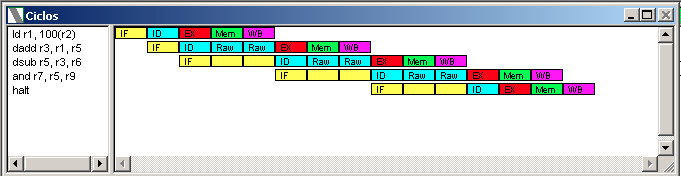
\includegraphics[scale=0.45]{raw.png}
\end{block}

\end{frame}


\subsection{WAR - Escritura luego de una Lectura}
\begin{frame}[fragile]
\frametitle{WAR}
Una instrucción escribe el valor de un registro antes que otra anterior que lo tiene que leer lo lea
\begin{block}{}
\begin{lstlisting}[language=WinMIPS64,basicstyle=\ttfamily,keywordstyle=\color{blue}]
.text ; Activar Forwarding

dmul r7,r1,r3
dmul r10,r7,r4
dadd r4,r5,r6
halt
\end{lstlisting}
\end{block}

\end{frame}


\begin{frame}[fragile]
\frametitle{WAR}
Una instrucción escribe el valor de un registro antes que otra anterior que lo tiene que leer lo lea
\begin{block}{}
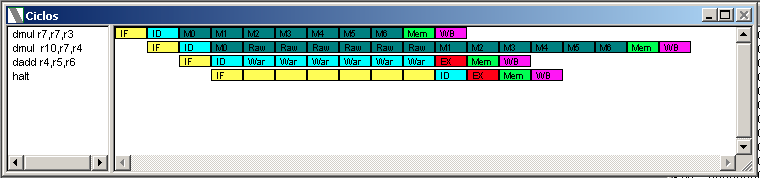
\includegraphics[scale=0.45]{war.png}
\end{block}
\end{frame}


\subsection{WAW - Escritura luego de una Escritura}
\begin{frame}[fragile]
\frametitle{WAW}
Una instrucción escribe un dato después que otra posterior
\begin{block}{}
\begin{lstlisting}[language=WinMIPS64,basicstyle=\ttfamily,keywordstyle=\color{blue}]
.text

dmul r1,r2,r3
dadd r1,r6,r3
halt
\end{lstlisting}
\end{block}

\end{frame}


\begin{frame}[fragile]
\frametitle{WAW}
Una instrucción escribe un dato después que otra posterior
\begin{block}{}
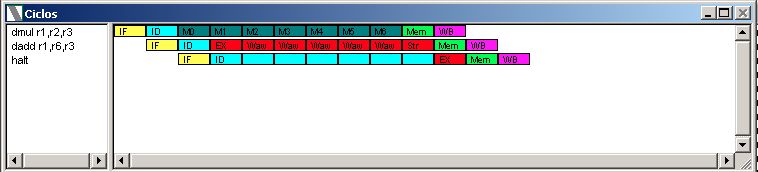
\includegraphics[scale=0.45]{waw.png}
\end{block}
\end{frame}

\section{Atascos por Dependencia de Control}
\subsection{General}
\begin{frame}[fragile]
\frametitle{General}
Una instrucción que modifica el valor del PC no lo ha hecho cuando se tiene que comenzar la siguiente.
\begin{itemize}
\item Estas instrucciones son saltos condicionales o incondicionales.
\item La decodificación de la instrucción se hace en el segundo ciclo de una instrucción, la siguiente instrucción ya ingreso en el cause en la etapa \emph{IF}.
\item Si el salto realmente se ejecuta, la próxima instrucción no sera la inmediata siguiente sino la que se determine por la instrucción
\end{itemize}
\begin{block}{}
\begin{lstlisting}[language=WinMIPS64,basicstyle=\ttfamily,keywordstyle=\color{blue}]
        .text
        j saltar
        dadd r1,r2,r3
saltar: halt
\end{lstlisting}
\end{block}
\end{frame}

\begin{frame}[fragile]
\frametitle{Atasco por Dependencia de Control}
\begin{block}{}
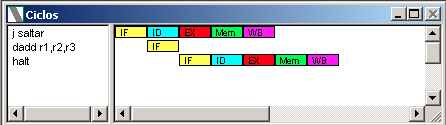
\includegraphics[scale=0.45]{atasco-branch-taken.png}
\end{block}
\end{frame}


\section{Posibles soluciones a riesgos estructurales}
\begin{frame}
\frametitle{Soluciones a riesgos estructurales}
Replicar, segmentar ó realizar turnos para el acceso a las unidades funcionales en conflicto.
\begin{itemize}
\item Duplicación de recursos hardware
\begin{itemize}
\item Unidades separadas para multiplicar, dividir además de la ALU
\end{itemize}
\item Separación en memorias de instrucciones y datos
\item Turnar el acceso al banco de registros
\begin{itemize}
\item Escrituras en la primera mitad de los ciclos de reloj
\item Lecturas en la segunda mitad de los ciclos de reloj
\end{itemize}
\end{itemize}
\end{frame}


\section{Posibles soluciones a problemas de dependencia de datos}
\begin{frame}
\frametitle{General}
\begin{itemize}
\item Se debe determinar cómo y cuando aparecen esos riesgos
\item Hay dos tipos de soluciones
\begin{itemize}
\item Software
\begin{itemize}
\item Podemos agregar instrucciones \emph{NOP}, o reordenar las instrucciones
\end{itemize}
\item Hardware
\begin{itemize}
\item Adelantamiento de Operandos (Forwarding)
\end{itemize}
\end{itemize}
\end{itemize}
\end{frame}

\subsection{Agregar NOPs}
\begin{frame}[fragile]
\frametitle{Agregar Instrucciones NOP}

Cambiemos el ejemplo visto anteriormente
\begin{block}{}
\begin{lstlisting}[language=WinMIPS64,basicstyle=\ttfamily,keywordstyle=\color{blue}]
.text
ld r1, 100(r2)
nop
nop
dadd r3, r1, r5
nop
nop
dsub r5, r3, r6
nop
nop
and r7, r5, r9
halt
\end{lstlisting}
\end{block}
Ahora no hay atascos, pero tenemos más instrucciones.
\end{frame}



\subsection{Reordenar instrucciones}
\begin{frame}[fragile]
\frametitle{Reordenar instrucciones}

Veamos otro ejemplo
\begin{block}{}
\begin{lstlisting}[language=WinMIPS64,basicstyle=\ttfamily,keywordstyle=\color{blue}]
.data
A: .word 5
.text
ld r1, A(r0)
dadd r1, r1, r1
daddi r2, r0, 3
dadd r3, r0, r0
halt
\end{lstlisting}
\end{block}
Tenemos un atasco con el registro \emph{r1}.

\end{frame}


\begin{frame}[fragile]
\frametitle{Reordenar instrucciones}
Retrasando el \emph{dadd} sobre el registro $r1$.
\begin{block}{}
\begin{lstlisting}[language=WinMIPS64,basicstyle=\ttfamily,keywordstyle=\color{blue}]
.data
A: .word 5
.text
ld r1, A(r0)
daddi r2, r0, 3
dadd r3, r0, r0
dadd r1, r1, r1
halt
\end{lstlisting}
\end{block}
No hay atascos ahora.
\end{frame}



\subsection{Forwarding}

\begin{frame}[fragile]
\frametitle{Forwarding}
Forwarding, Adelantamiento o Cortocircuito
\begin{itemize}
\item Consiste en pasar directamente el resultado obtenido con una instrucción a las instrucciones que lo necesitan como operando.
\item Si el dato necesario está disponible antes se lleva a la entrada de la etapa correspondiente sin esperar a llegar a la etapa escritura de escritura del banco de registros.
\item La idea es tener disponible el operando lo antes posible para no perder ciclos
\item Usar esta técnica no implica la eliminación de todos los atascos.
\item En WinMIPS64 podemos activarlo o desactivarlo en cualquier momento. Un cambio en esta configuración implica reiniciar la simulación.
\end{itemize}
\end{frame}


\begin{frame}[fragile]
\frametitle{Forwarding}
Forwarding, Adelantamiento o Cortocircuito
\begin{itemize}
\item Cuando no existe Forwarding, una instrucción debe tener todos sus operandos (registros) disponibles en la etapa ID
\item Cuando esta activo los registros pueden aelantarse una vez calculados o leidos a la etapa que los necesita. No siempre esa etapa es ID.
\item Que instrucciones pueden adelantar un operando:
\begin{itemize}
\item Si la instrucción es de lectura de memoria, puede adelantar el operando luego de ejecutar la etapa MEM.
\item Si es una instrucción aritmetico / lógica, luego de ejecutada la etapa EX.
\end{itemize}
\item Si el operando se podia adelantar en EX, podrá también adelantarlo en MEM si una instrucción lo requiere.
\end{itemize}
\end{frame}

\begin{frame}[fragile]
\frametitle{Forwarding}
Forwarding, Adelantamiento o Cortocircuito
\begin{itemize}
\item Cuando se requiere un operando:
\begin{itemize}
\item Si la instrucción es de escritura de memoria, el operando a escribir, se necesita en MEM.
\item Si el operando se necesita para una operación aritmetico / lógica, se necesita en la etapa EX.
\item Si el operando se necesita para una instrucción de salto condicional, se necesita en la etapa ID.
\end{itemize}
\end{itemize}
\end{frame}

\begin{frame}[fragile]
\frametitle{Forwarding}
Forwarding, Adelantamiento o Cortocircuito
\begin{itemize}
\item Situaciones donde pueden ocurrir forwarding
\begin{itemize}
\item Lectura seguida de Escritura
\item Lectura seguida de Aritmetico / Lógica
\item Lectura seguida de Salto Condicional
\item Aritmetica / Lógica seguida de Escritura
\item Aritmetica / Lógica seguida de Aritmetico / Logica
\item Aritmetica / Lógica seguida de Salto Condicional
\item Lectura seguida de Lectura 
\item Aritmetica / Lógica seguida de Lectura
\end{itemize}
\end{itemize}
\end{frame}


\begin{frame}[fragile]
\frametitle{Forwarding - Lectura seguida de escritura}
\begin{itemize}
\item Lectura seguida de Escritura
\begin{itemize}
\item El operando a escribir en memoria viene de una instrucción de lectura anterior.
\item La instrucción \emph{sd} debe esperar a que la instrucción \emph{ld} se complete, esperando en \emph{ID}
\end{itemize}
\end{itemize}
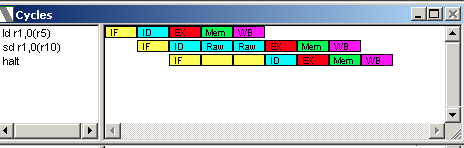
\includegraphics[scale=0.45]{forwarding-1.png}
\end{frame}

\begin{frame}[fragile]
\frametitle{Forwarding - Lectura seguida de escritura}
\begin{itemize}
\item Lectura seguida de Escritura
\begin{itemize}
\item Con el adelantamiento activo, cuando la instrucción \emph{ld} pasa la etapa \emph{MEM}, ya puede adelantar el operando
\item La instrucción \emph{sd} necesita el registro r1 en la etapa de \emph{MEM}
\item Por lo tanto ya no hay atascos RAW.
\end{itemize}
\end{itemize}
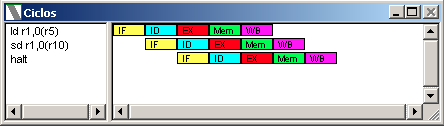
\includegraphics[scale=0.45]{forwarding-1-lectura-escritura.png}
\end{frame}


\begin{frame}[fragile]
\frametitle{Forwarding - Lectura seguida de Aritmetico / Logica}
\begin{itemize}
\item Lectura seguida de Aritmetico / Lógica
\begin{itemize}
\item Uno de los operandos de una instrucción aritmetico lógico proviene de una lectura de memoria
\item La instrucción \emph{daddi} debe esperar a que la instrucción \emph{ld} se complete, esperando en \emph{ID}
\end{itemize}
\end{itemize}
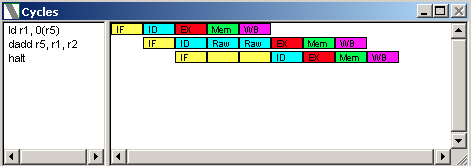
\includegraphics[scale=0.45]{forwarding-2.png}
\end{frame}

\begin{frame}[fragile]
\frametitle{Forwarding - Lectura seguida de Aritmetico / Logica}
\begin{itemize}
\item Lectura seguida de Aritmetico / Lógica
\begin{itemize}
\item Con el adelantamiento activo, cuando la instrucción \emph{ld} pasa la etapa \emph{MEM}, ya puede adelantar el operando
\item La instrucción \emph{daddi} necesita el registro r1 en la etapa de \emph{EX}
\item Como \emph{daddi} debe esperar en \emph{EX} a que \emph{ld} pase la etapa \emph{MEM}, se produce un solo atasco RAW.
\end{itemize}
\end{itemize}
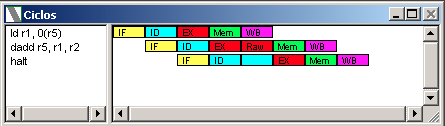
\includegraphics[scale=0.45]{forwarding-2-lectura-aritm.png}
\end{frame}


\begin{frame}[fragile]
\frametitle{Forwarding - Lectura seguida de Salto Condicional}
\begin{itemize}
\item Lectura seguida de Salto Condicional
\begin{itemize}
\item Uno de los operandos de una instrucción de salto condicional proviene de una lectura de memoria
\item La instrucción \emph{beqz} debe esperar a que la instrucción \emph{ld} se complete, esperando en \emph{ID}
\end{itemize}
\end{itemize}
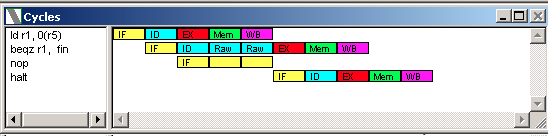
\includegraphics[scale=0.45]{forwarding-3.png}
\end{frame}

\begin{frame}[fragile]
\frametitle{Forwarding - Lectura seguida de Salto Condicional}
\begin{itemize}
\item Lectura seguida de Salto Condicional
\begin{itemize}
\item Con el adelantamiento activo, cuando la instrucción \emph{ld} pasa a la etapa \emph{MEM}, ya puede adelantar el operando
\item La instrucción \emph{beqz} necesita el registro r1 en la etapa de \emph{ID}
\item Por lo tanto esta situación no cambia
\end{itemize}
\end{itemize}
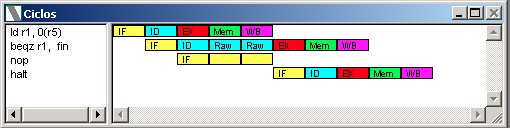
\includegraphics[scale=0.45]{forwarding-3-lectura-beq.png}
\end{frame}


\begin{frame}[fragile]
\frametitle{Forwarding - Aritmetica / Lógica seguida de Escritura}
\begin{itemize}
\item Aritmetica / Lógica seguida de Escritura
\begin{itemize}
\item El operando a escribir en memoria viene de una instrucción aritmetico lógica anterior.
\item La instrucción \emph{sd} debe esperar a que la instrucción \emph{daddi} se complete, esperando en \emph{ID}
\end{itemize}
\end{itemize}
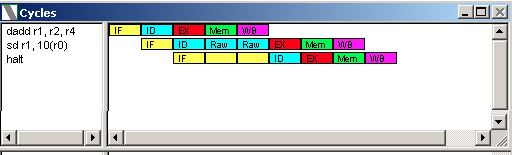
\includegraphics[scale=0.45]{forwarding-4.png}
\end{frame}

\begin{frame}[fragile]
\frametitle{Forwarding - Aritmetica / Lógica seguida de Escritura}
\begin{itemize}
\item Aritmetica / Lógica seguida de Escritura
\begin{itemize}
\item Con el adelantamiento activo, cuando la instrucción \emph{daddi} pasa la etapa \emph{EX}, ya puede adelantar el operando
\item La instrucción \emph{sd} necesita el registro r1 en la etapa de \emph{MEM}
\item Por lo tanto ya no hay atascos RAW.
\end{itemize}
\end{itemize}
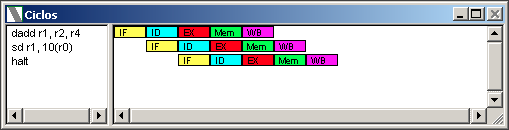
\includegraphics[scale=0.45]{forwarding-4-aritmetica-escritura.png}
\end{frame}

\begin{frame}[fragile]
\frametitle{Forwarding - Aritmetica / Lógica seguida de Aritmetico / Logica}
\begin{itemize}
\item Aritmetica / Lógica seguida de Aritmetico / Logica
\begin{itemize}
\item Un operando de una instrucción aritmetico lógica viene de una instrucción aritmetico lógica anterior.
\item La segunda  instrucción \emph{daddi} debe esperar a que la primer instrucción \emph{daddi} se complete, esperando en \emph{ID}
\end{itemize}
\end{itemize}
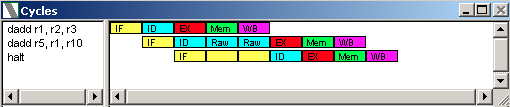
\includegraphics[scale=0.45]{forwarding-5.png}
\end{frame}

\begin{frame}[fragile]
\frametitle{Forwarding - Aritmetica / Lógica seguida de Aritmetico / Logica}
\begin{itemize}
\item Aritmetica / Lógica seguida de Aritmetico / Logica
\begin{itemize}
\item Con el adelantamiento activo, cuando la primer instrucción \emph{daddi} pasa la etapa \emph{EX}, ya puede adelantar el operando
\item La segunda instrucción \emph{daddi} necesita el registro r1 en la etapa de \emph{EX}
\item Por lo tanto ya no hay atascos RAW.
\end{itemize}
\end{itemize}
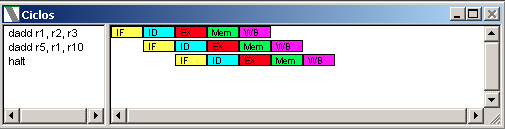
\includegraphics[scale=0.45]{forwarding-5-aritmetica-aritmetica.png}
\end{frame}


\begin{frame}[fragile]
\frametitle{Forwarding - Aritmetica / Lógica seguida de Salto Condicional}
\begin{itemize}
\item Aritmetica / Lógica seguida de Salto Condicional
\begin{itemize}
\item Un operando de una instrucción de salto condicional viene de una instrucción aritmetico lógica anterior.
\item La instrucción \emph{beqz} debe esperar a que la instrucción \emph{daddi} se complete, esperando en \emph{ID}
\end{itemize}
\end{itemize}
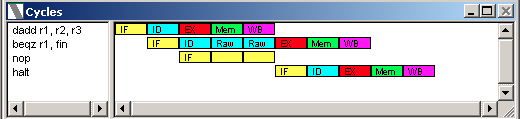
\includegraphics[scale=0.45]{forwarding-6.png}
\end{frame}

\begin{frame}[fragile]
\frametitle{Forwarding - Aritmetica / Lógica seguida de Salto Condicional}
\begin{itemize}
\item Aritmetica / Lógica seguida de Salto Condicional
\begin{itemize}
\item Con el adelantamiento activo, cuando la instrucción \emph{daddi} pasa la etapa \emph{EX}, ya puede adelantar el operando
\item La instrucción \emph{beqz} necesita el registro r1 en la etapa de \emph{ID}
\item Como \emph{beqz} debe esperar en \emph{ID} a que \emph{daddi} pase la etapa \emph{EX}, se produce un solo atasco RAW.
\end{itemize}
\end{itemize}
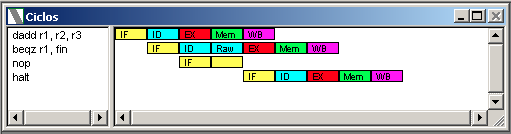
\includegraphics[scale=0.45]{forwarding-6-aritmetica-salto-condicional.png}
\end{frame}

\begin{frame}[fragile]
\frametitle{Forwarding - Lectura seguida de Lectura}
\begin{itemize}
\item Lectura seguida de Lectura
\begin{itemize}
\item El operando que calcula el desplazamiento en memoria de una escritura viene de una instrucción de lectura anterior.
\item La segunda instrucción \emph{ld} debe esperar a que la primer instrucción \emph{ld} se complete, esperando en \emph{ID}
\end{itemize}
\end{itemize}
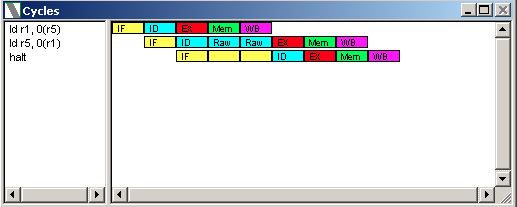
\includegraphics[scale=0.45]{forwarding-7.png}
\end{frame}

\begin{frame}[fragile]
\frametitle{Forwarding - Lectura seguida de Lectura}
\begin{itemize}
\item Lectura seguida de Lectura
\begin{itemize}
\item Con el adelantamiento activo, cuando la primer instrucción \emph{ld} pasa la etapa \emph{MEM}, ya puede adelantar el operando
\item La segunda instrucción \emph{ld} necesita acceder a r1 en la etapa \emph{EX}
\item Como la segunda instrucción \emph{ld} debe esperar en \emph{EX} a que la primer instrucción  \emph{ld} pase la etapa \emph{MEM}, se produce un solo atasco RAW.

\end{itemize}
\end{itemize}
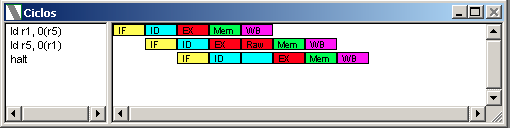
\includegraphics[scale=0.45]{forwarding-7-lectura-lectura.png}
\end{frame}


\begin{frame}[fragile]
\frametitle{Forwarding - Aritmetica / Lógica seguida de Lectura}
\begin{itemize}
\item Aritmetica / Lógica seguida de Lectura
\begin{itemize}
\item El operando que calcula el desplazamiento en memoria de una escritura viene de una instrucción aritmetico lógica anterior.
\item La instrucción \emph{ld} debe esperar a que la instrucción \emph{daddi} se complete, esperando en \emph{ID}
\end{itemize}
\end{itemize}
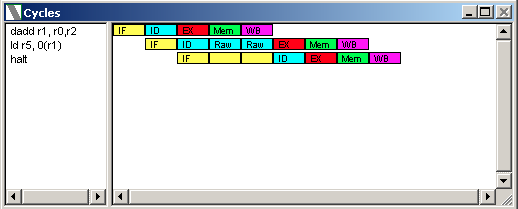
\includegraphics[scale=0.45]{forwarding-8.png}
\end{frame}

\begin{frame}[fragile]
\frametitle{Forwarding - Aritmetica / Lógica seguida de Lectura}
\begin{itemize}
\item Aritmetica / Lógica seguida de Lectura
\begin{itemize}
\item Con el adelantamiento activo, cuando la instrucción \emph{daddi} pasa la etapa \emph{EX}, ya puede adelantar el operando
\item La instrucción \emph{ld} necesita acceder a r1 en la etapa \emph{EX}
\item Por lo tanto ya no hay atascos RAW.
\end{itemize}
\end{itemize}
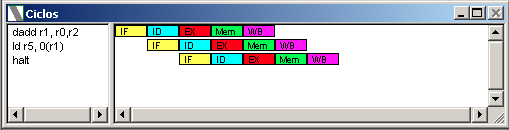
\includegraphics[scale=0.45]{forwarding-8-aritmetica-lectura.png}
\end{frame}


\section{Posibles soluciones a problemas de dependencia de control}
\begin{frame}
\frametitle{General}
Existe una Penalización por salto, ya que se empieza a analizar la instrucción inmediata siguiente, mientras estamos decodificando el salto. Las instrución de salto puede ser: 
\begin{itemize}
\item Incondicional: La dirección de destino se debe determinar lo más pronto posible, dentro del cauce, para reducir la penalización.
\item Condicional: Introduce riesgo adicional por la dependencia entre la condición de salto y el resultado de una instrucción previa.
\end{itemize}
Deberiamos encontrar alguna manera de saber cual es la próxima instrucción lo antes posible.
\end{frame}


\subsection{Branch Target Buffer}
\begin{frame}
\frametitle{Branch-Target-Buffer}
Podemos ir guardando un historial de saltos para poder "predecir" si un salto se produce o no.
\begin{itemize}
\item Cada vez que se ejecuta una instrucción de salto se guarda un registro si el salto se realizo o no (un registro para cada instrucción de salto). Ejemplo:
\begin{itemize}
\item Tengo un contador, inicialmente en 0. Sumo 1 por salto realizado, resto 1 si el salto no se realiza.
\item La próxima vez que pasé por esa instrucción puedo \emph{predecir} si el salto se realizará o no. 
\item Si el contador es positivo asumo se realizara el salto, la próxima instrucción será la que resulte de ejecutar el salto
\item Si el contador fuera negativo asumo no se realiza el salto, la próxima instrucción será la siguiente.
\end{itemize}
\item Que se hace la primera vez que se evalua un salto depende de la arquitectura.
\end{itemize}
\end{frame}

\begin{frame}
\frametitle{Branch-Target-Buffer en el Simulador}
\begin{itemize}
\item El simulador WinMIPS64 permite activar o desactivar la predicción de Saltos
\item La predicción de saltos usado en el simulador funciona de la siguiente manera:
\begin{itemize}
\item Si es la primera vez que se realiza el salto, se predice que el salto no va a ocurrir.
\item Si la instrucción se ejecuto por lo menos una vez, se asume que va a ocurrir lo último que ocurrió.
\item Si el resultado de la predicción cambio, se actualiza ese estado.
\end{itemize}
\item Si una predicción no ocurre, hay una penalidad de un ciclo perdido adicional.\end{itemize}
\end{frame}


\begin{frame}
\frametitle{Branch-Target-Buffer en el Simulador}
\begin{itemize}
\item Si un salto se predice que va a ocurrir y no ocurre. La penalidad son 2 atascos Branch Misprediction.
\item Si un salto se predice que no va a ocurrir y ocurre. La penalidad son 2 atascos Branch Taken.
\item Los 2 atascos corresponden a:
\begin{itemize}
\item 1 Ciclo para la actualización de la tabla BTB
\item 1 Ciclo para la carga de la nueva instrucción (como ocurria sin BTB)
\end{itemize}
\end{itemize}
\end{frame}

\begin{frame}
\frametitle{Branch-Target-Buffer en el Simulador}
\begin{itemize}
\item Si un salto se predice que va a ocurrir, podemos ver un simbolo después de la dirección de memoria en la ventana del programa
\end{itemize}
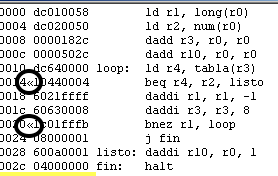
\includegraphics[scale=0.65]{btb.png}
\end{frame}


\subsection{Delay Slot}
\begin{frame}
\frametitle{Delay Slot}
Salto retardado o de relleno de ranura de retardo
\begin{itemize}
\item Es un método alternativo de atacar el problema de los atascos por dependencia de Control
\item El problema es la predicción de la siguiente instrucción luego de un salto.
\item Delay Slot ofrece como solución que la siguiente instrucción después de un salto \emph{SIEMPRE} se ejecute.
\item Esto elimina el problema de la predicción de instrucciones...
\item ... pero hay que tener en cuenta a la hora de programar.

\end{itemize}
\end{frame}

\begin{frame}[fragile]
\frametitle{Delay Slot}
¿Es lo mismo con o sin \emph{Delay Slot}?
\begin{block}{}
\begin{lstlisting}[language=WinMIPS64,basicstyle=\ttfamily,keywordstyle=\color{blue}]
       .data
A:   .word 2
       .text
       ld    r1, A(r0)
       daddi r2, r0, 3
       dadd  r3, r0, r0
salto: dadd  r3, r3, r1
       daddi r2, r2, -1
       bnez  r2, salto
       halt
\end{lstlisting}
\end{block}
\end{frame}


\begin{frame}[fragile]
\frametitle{Delay Slot - Solución 1 }
Podemos ``arreglar'' nuestro programa poniendo un \emph{NOP}, luego del salto.
\begin{block}{}
\begin{lstlisting}[language=WinMIPS64,basicstyle=\ttfamily,keywordstyle=\color{blue}]
       .data
A:   .word 2
       .text
       ld    r1, A(r0)
       daddi r2, r0, 3
       dadd  r3, r0, r0
salto: dadd  r3, r3, r1
       daddi r2, r2, -1
       bnez  r2, salto
       nop
       halt
\end{lstlisting}
\end{block}
\end{frame}


\begin{frame}[fragile]
\frametitle{Delay Slot - Solución 2 }
O podriamos reordenar las instrucciones...
\begin{block}{}
\begin{lstlisting}[language=WinMIPS64,basicstyle=\ttfamily,keywordstyle=\color{blue}]
       .data
A:   .word 2
       .text
       ld    r1, A(r0)
       daddi r2, r0, 3
       dadd  r3, r0, r0
salto: daddi  r2, r2, -1
       bnez  r2, salto
       dadd r3, r3, r1
       halt
\end{lstlisting}
\end{block}
\end{frame}


\begin{frame}
\frametitle{Delay Slot en el Simulador}
\begin{itemize}
\item El simulador WinMIPS64 permite activar o desactivar el Delay Slot
\item No se pueden tener activos Delay-Slot y Branch-Target-Buffer al mismo tiempo
\item Recordar que cualquier cambio en estas opciones involucra un reinicio en la simulación
\end{itemize}
\end{frame}


\end{document}

